\begin{figure}
    \centering
    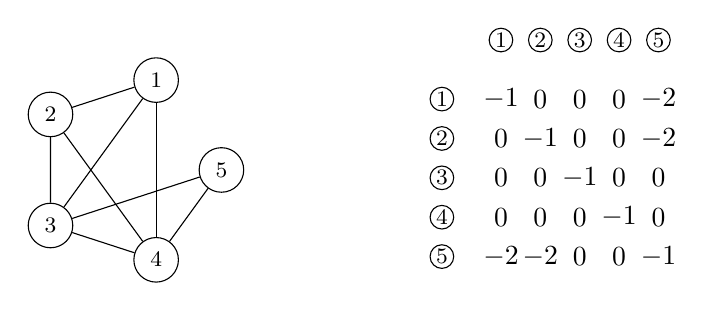
\begin{tikzpicture}

        % Graph on the left (smaller size)
        \begin{scope}[xshift=-3cm, yshift=.6cm, scale=0.8]
            % Nodes
            \foreach \i in {1, 2, 3, 4, 5} {
                \node[circle, draw, minimum size=0.3cm, font=\footnotesize] (v\i) at (360/5 * \i:1.5) {\i};
            }

            % Edges (all but two edges)
            \draw (v1) -- (v2);
            \draw (v1) -- (v3);
            \draw (v1) -- (v4);
            \draw (v2) -- (v3);
            \draw (v2) -- (v4);
            \draw (v3) -- (v4);
            \draw (v3) -- (v5);
            \draw (v4) -- (v5);
        \end{scope}

        % Adjacency matrix on the right (aligned with the graph)
        \begin{scope}[xshift=1.5cm, yshift=-0.75cm]
            % Labels for rows and columns (circled nodes)
            \foreach \i in {1, 2, 3, 4, 5} {
                % Row labels (left side)
                \node[circle, draw, minimum size=0.3cm, font=\footnotesize,inner sep=0pt] at (-0.5, 2.5 - 0.5*\i + 0.25) {\i};
                % Column labels (top side)
                \node[circle, draw, minimum size=0.3cm, font=\footnotesize,inner sep=0pt] at (0.5*\i - 0.25, 3.0) {\i};
            }

            % Manually fill in the adjacency matrix
            % Row 1
            \node at (0.25, 2.25) {$-1$}; % (1,1)
            \node at (0.75, 2.25) {$0$};  % (1,2)
            \node at (1.25, 2.25) {$0$};  % (1,3)
            \node at (1.75, 2.25) {$0$};  % (1,4)
            \node at (2.25, 2.25) {$-2$}; % (1,5)

            % Row 2
            \node at (0.25, 1.75) {$0$};  % (2,1)
            \node at (0.75, 1.75) {$-1$}; % (2,2)
            \node at (1.25, 1.75) {$0$};  % (2,3)
            \node at (1.75, 1.75) {$0$};  % (2,4)
            \node at (2.25, 1.75) {$-2$}; % (2,5)

            % Row 3
            \node at (0.25, 1.25) {$0$};  % (3,1)
            \node at (0.75, 1.25) {$0$};  % (3,2)
            \node at (1.25, 1.25) {$-1$}; % (3,3)
            \node at (1.75, 1.25) {$0$};  % (3,4)
            \node at (2.25, 1.25) {$0$};  % (3,5)

            % Row 4
            \node at (0.25, 0.75) {$0$};  % (4,1)
            \node at (0.75, 0.75) {$0$};  % (4,2)
            \node at (1.25, 0.75) {$0$};  % (4,3)
            \node at (1.75, 0.75) {$-1$}; % (4,4)
            \node at (2.25, 0.75) {$0$};  % (4,5)

            % Row 5
            \node at (0.25, 0.25) {$-2$}; % (5,1)
            \node at (0.75, 0.25) {$-2$}; % (5,2)
            \node at (1.25, 0.25) {$0$};  % (5,3)
            \node at (1.75, 0.25) {$0$};  % (5,4)
            \node at (2.25, 0.25) {$-1$}; % (5,5)
        \end{scope}

    \end{tikzpicture}
    \caption{An example of matrix $\mat{A} = \mat{A}(G)$ (right) for graph $G$ (left).}
    \label{fig:graph}
\end{figure}